%% 03.tex
\documentclass[platex,dvipdfmx]{jsreport}

\usepackage{graphicx}
\graphicspath{{./images/}{../images/}}
\usepackage{pdfpages}
\usepackage{tikz}
\usepackage{xcolor}
\definecolor{UD_GREEN}{HTML}{03af7a}
\usepackage{bm}
\usepackage[left=30truemm]{geometry}
\usepackage{amsmath,amssymb}
\numberwithin{equation}{section}



\begin{document}

\chapter{本論}

\section{手法}
\subsection{逆オパール構造}
逆オパール構造の球の半径$r / a$を徐々に変化させていった際のバンドギャップの変化を観察した。このときのバンドギャップの変化を$\epsilon = 5, 10, 13, 15$のそれぞれについて行い、各$\epsilon$におけるバンドギャップの数とギャップ-ミッドギャップ比の変化を観察し最適な構造を検討した。
\subsection{ウッドパイル構造}
ウッドパイル構造の誘電体棒の幅$w / a$を徐々に変化させていった際のバンドギャップの変化を観察した。このときのバンドギャップの変化を$\epsilon = 5, 10, 13, 15$のそれぞれについて行い、各$\epsilon$におけるバンドギャップの数とギャップ-ミッドギャップ比の変化を観察し最適な構造を検討した。
\subsection{ヤブロノバイト構造}
ヤブロノバイト構造の誘電体円柱の半径$r / a$を徐々に変化させていった際のバンドギャップの変化を観察した。このときのバンドギャップの変化を$\epsilon = 5, 10, 13, 15$のそれぞれについて行い、各$\epsilon$におけるバンドギャップの数とギャップ-ミッドギャップ比の変化を観察し最適な構造を検討した。
\subsection{2次元構造の積み重ね}
2次元結晶の積み重ねにより作成された3次元構造の空気柱の半径$r / a$を徐々に変化させていった際のバンドギャップの変化を観察した。このときのバンドギャップの変化を$\epsilon = 5, 10, 12, 15$のそれぞれについて行い、各$\epsilon$におけるバンドギャップの数とギャップ-ミッドギャップ比の変化を観察し最適な構造を検討した。


\section{結果}
\subsection{逆オパール構造}
逆オパール構造に配置されている球の半径$r / a$を0.01ずつ変化させ、ギャップ-ミッドギャップ比の変化を観察した。この変化を$\epsilon = 5, 10, 13, 15$のそれぞれについて行った。

このときの各$\epsilon$におけるギャップマップを以下の図\ref{fig:gapmap_inv_opal_e-5}から図\ref{fig:gapmap_inv_opal_e-15}に示す。

\begin{figure}[h]
  \begin{minipage}[h]{0.5\linewidth}
    \centering
    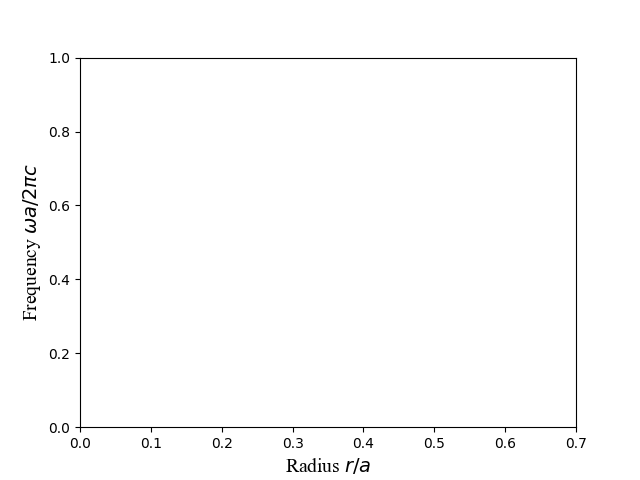
\includegraphics[keepaspectratio, scale=0.45]{results/gap_map/inv_e-5.png}
    \caption{逆オパール構造のギャップマップ($\epsilon = 5$)}
    \label{fig:gapmap_inv_opal_e-5}
  \end{minipage}
  \begin{minipage}[h]{0.5\linewidth}
    \centering
    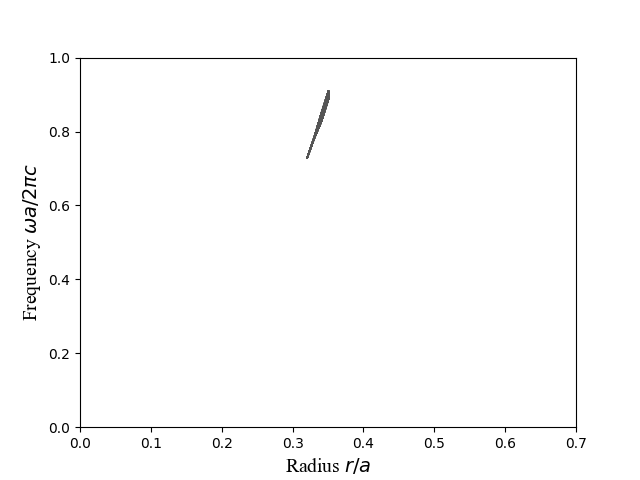
\includegraphics[keepaspectratio, scale=0.45]{results/gap_map/inv_e-10.png}
    \caption{逆オパール構造のギャップマップ($\epsilon = 10$)}
    \label{fig:gapmap_inv_opal_e-10}
  \end{minipage}
  \begin{minipage}[h]{0.5\linewidth}
    \centering
    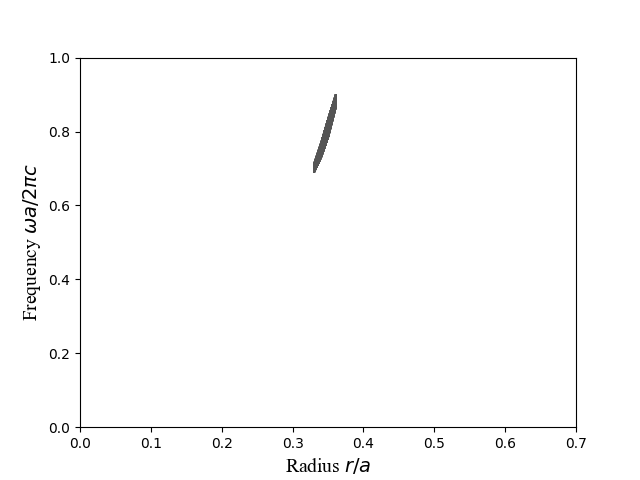
\includegraphics[keepaspectratio, scale=0.45]{results/gap_map/inv_e-13.png}
    \caption{逆オパール構造のギャップマップ($\epsilon = 13$)}
    \label{fig:gapmap_inv_opal_e-13}
  \end{minipage}
  \begin{minipage}[h]{0.5\linewidth}
    \centering
    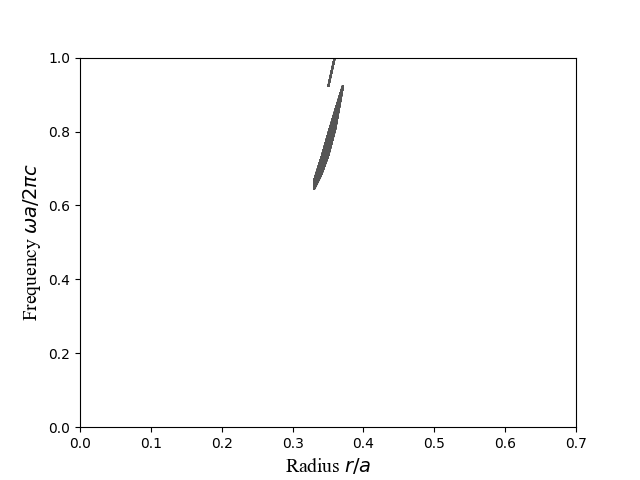
\includegraphics[keepaspectratio, scale=0.45]{results/gap_map/inv_e-15.png}
    \caption{逆オパール構造のギャップマップ($\epsilon = 15$)}
    \label{fig:gapmap_inv_opal_e-15}
  \end{minipage}
\end{figure}

$\epsilon = 5$のとき、バンドギャップは生じなかった。一方で$\epsilon = 10, 13, 15$のときはバンドギャップが生じた。$\epsilon = 10, 13$のときはバンドギャップは1つであったが、$\epsilon = 15$のときはバンドギャップは2つであった。

次に、各$\epsilon$において球の半径とギャップ-ミッドギャップ比の関係を図\ref{fig:inv_opal}に示す。

  
\begin{figure}[htbp]
  \centering
  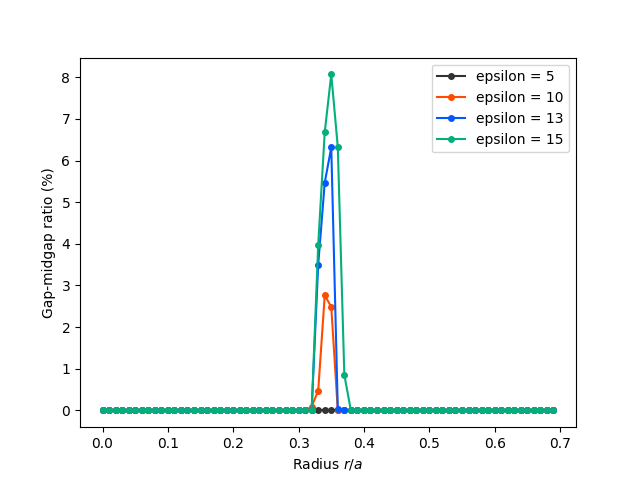
\includegraphics[width=0.8\linewidth]{results/gap_midgap_ratio/inv_opals.png}
  \caption{逆オパール構造の球の半径を変化させた際のギャップ-ミッドギャップ比の変化}
  \label{fig:inv_opal}
\end{figure}





$\epsilon = 5$のときはバンドギャップは確認できなかった。

$\epsilon = 13$のとき、$0.34 \leq r / a \leq 0.37$の範囲でのみバンドギャップが確認でき、その中で最大値をとる$r / a = 0.36$のときのギャップ-ミッドギャップ比は最大となりその値は$6.41675 \% $であった。



\subsection{ウッドパイル構造}
ウッドパイル構造中の棒状誘電体の幅を徐々に変化させていった際のギャップ-ミッドギャップ比の変化を図\ref{fig:woodpile}に示す。

\begin{figure}[htbp]
  \centering
  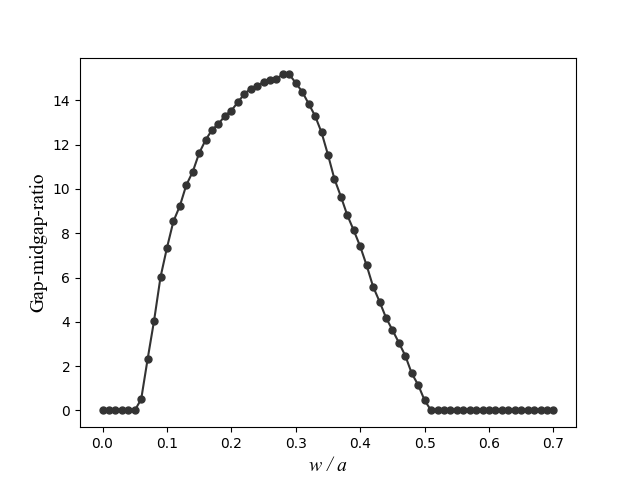
\includegraphics[width=0.6\linewidth]{results/woodpile.png}
  \caption{ウッドパイル構造の棒状誘電体の幅を変化させた際のギャップ-ミッドギャップ比の変化}
  \label{fig:woodpile}
\end{figure}

誘電体棒幅$w = 0.28$で最大となり、ギャップ-ミッドギャップ比は$15.17613425 \%$となった。

\subsection{ヤブロノバイト構造}
ヤブロノバイト構造中の空気柱の半径を連続的に変化させた際のギャップ-ミッドギャップ比の変化を図\ref{fig:yablonovite}に示す。
\begin{figure}[htbp]
  \centering
  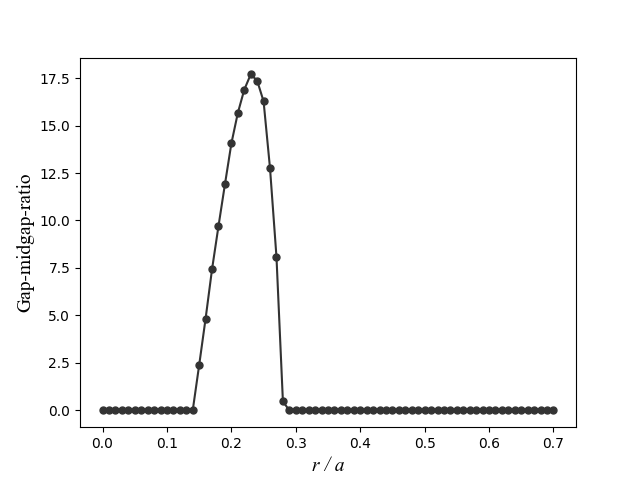
\includegraphics[width=0.6\linewidth]{results/yablonovite.png}
  \caption{ヤブロノバイト構造の空気柱の半径を変化させた際のギャップ-ミッドギャップ比の変化}
  \label{fig:yablonovite}
\end{figure}

空気中の半径$r / a = 0.23$でギャップ-ミッドギャップ比は最大となり、その値は$17.6924 \%$だった。

\subsection{2次元構造の積み重ね}
2次元結晶の積み重ねによって3次元結晶を作成した際のギャップ-ミッドギャップ比の変化を図\ref{fig:stack-crystals}に示す。
\begin{figure}[htbp]
  \centering
  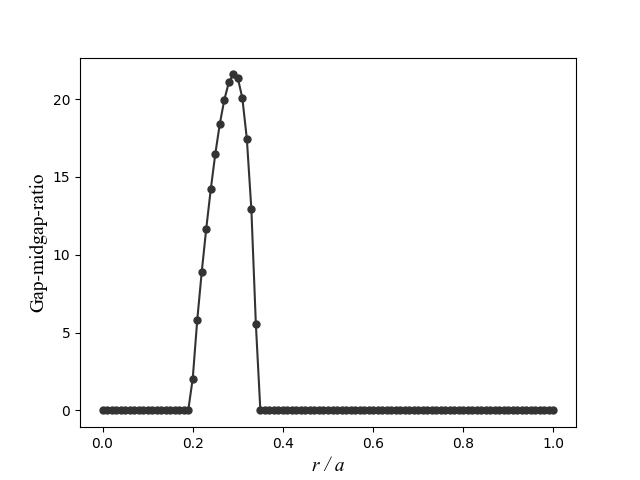
\includegraphics[width=0.6\linewidth]{results/stack-crystals.png}
  \caption{2次元結晶の積み重ねによって作成した3次元結晶のギャップ-ミッドギャップ比の変化}
  \label{fig:stack-crystals}
\end{figure}
半径$r / a = 0.29$の球を2次元結晶として積み重ねた際に最大となり、ギャップ-ミッドギャップ比は$21.58 \%$となった。



\end{document}